\documentclass[10pt,journal,compsoc]{IEEEtran}
\usepackage[brazilian]{babel}
\usepackage[utf8]{inputenc}
\usepackage{graphicx}

\usepackage{minted}
\usepackage{xcolor}
\definecolor{LightGray}{gray}{0.9}
\definecolor{DarkGray}{gray}{0.1}
\usemintedstyle{monokai}


\begin{document}

\title{Password Cracking \\ Processamento Paralelo}

\author{André~Thiago~Borghi~Couto,~\IEEEmembership{Graduando,~UFES}
        \\ Bruno~Calmon~Barreto,~\IEEEmembership{Graduando,~UFES}%
    \IEEEcompsocitemizethanks{
        \IEEEcompsocthanksitem A.T.B. Couto está graduando em ciência da computação, na UFES, campus CEUNES, em São Mateus - ES.\protect\\
            E-mail: andreww.max@hotmail.com
        \IEEEcompsocthanksitem B.C. Barreto está graduando em ciência da computação, na UFES, campus CEUNES, em São Mateus - ES.\protect\\
            E-mail: bruno****************************
        }
    \thanks{Trabalho escrito em 1 de julho de 2019;}
}
\markboth{\LaTeX\ UFES - Processamento Paralelo,~Vol.~2, EP.~2, Julho~2019}
{Couto \MakeLowercase{\textit{et al.}}: Estudo para a criação paralelizada de quebra de senhas com MPI}

\IEEEtitleabstractindextext{
    \begin{abstract}
        % Senhas são atualmente umas das coisas mais importantes para cada ser humano que vive neste mundo, sabendo que com uma dessas senhas é possível ter todas informações da vida de uma pessoa em suas mãos, pessoas mal intencionadas podem querer fazer proveito disto, com todos os métodos de criptografia existentes atualmente, que tentam deixar-nos mais seguros quanto a ataques, mas e como fazer isto, como descobrir uma senha criptografada? Neste trabalho apresentaremos uma forma de obter certas senhas. 
        Passwords are currently one of the most important things for every human being living in this world, knowing that with one of these passwords it is possible to have all the information of a person's life in their hands, malicious people may want to take advantage of this with all methods encryption algorithms that currently exist that try to make us safer for attacks, but how to do this, how to find an encrypted password? In this work we will present a way to obtain certain passwords.
    \end{abstract}
    \begin{IEEEkeywords}
        Computer Science, Parallel Processing, Comunnications, Password Cracking, \LaTeX, Ciência da Computação, MPI, Processamento Paralelo.
    \end{IEEEkeywords}
}

\maketitle
\IEEEdisplaynontitleabstractindextext
\IEEEpeerreviewmaketitle
\IEEEraisesectionheading{
\section{Introdução}
\label{sec:introducao}
}
\IEEEPARstart{S}{e} pudéssemos descrever um problema desafiador em nossa vida, esse problema seria lembrar todas as senhas, que atualmente são de suma importância para nosso cotidiano, seja virtualmente (redes sociais, jogos, aplicativos) ou reais (bancos ou cadeados), mesmo tomando todos os cuidados ainda estamos vulneráveis aos ataques de quebra (cracking) de senhas, assim, todo cuidado é pouco, pois se temos senhas simples, ou muito usadas, elas podem ser facilmente descobertas.

O trabalho em si é um exemplo de ataque de força bruta, no qual é aplicado sequencialmente todas as permutações de uma determinada quantidade de caracteres que por sua vez é criptografada e comparada à que foi passada para ser descoberta.

\section{Estratégia}
\label{sec:estrategia}
Primeiramente nosso código foi escrito em C++, utilizando a biblioteca MPI e técnicas da mesma, que são para a paralelização do código em nível de processo, como o fork.

Nossa estratégia consiste em dividir em um limite dentro do vetor dos caracteres, utilizando a divisão pela quantidade de Processadores para definir o início de cada um deles, assim cada processador recebe \mintinline[style=bash, bgcolor=LightGray]{c}{strlen(caracteres) / np} no qual devemos discutir abaixo pelo código. Mais adiante teremos as opções para discutir, uma delas leva em consideração que o $Processador~0$, não faz os cálculos, então deve-se admitir que cada Processador recebe \mintinline[style=bash, bgcolor=LightGray]{c}{strlen(caracteres) / (np - 1)}.

Para começarmos temos o básico em receber os dados de entrada ou seja a senha que vai ser quebrada, em seguida criamos a String de resposta, juntamente com a declaração dos caracteres que serão utilizados, isso permite definir qual a complexidade da senha a ser quebrada, logo para este trabalho utilizaremos o básico, alfabeto minúsculo e maiúsculo além dos números. Em seguida temos opções do MPI, que são $np$, como número de processadores e $rank$ como o número do atual processador, sendo o principal $0$ e os demais distribuídos de forma incremental. Visto que MPI possui seus próprios métodos para manipulação de processos, a $MPI\_Init$ representa o início do código para o MPI, $MPI\_Comm\_rank$ representa o numero do processador atual, e $MPI\_Comm\_size$ representa a quantidade de processadores, no caso essa informação é externa, que é passada na execução do $mpirun -np~\#$, onde $\#$ é o número desejado de processadores.

\begin{minted}[frame=lines, bgcolor=DarkGray, fontsize=\footnotesize, framesep=2mm, baselinestretch=1.2, breaklines, breakanywhere, autogobble]{c++}
int main(int argc, char *argv[]) {
    
    char *SENHA = argv[1];
    char *RESPOSTA;
    char caracteres[] = "abcdefghijklmnopqrstuvwxyzABCDEFGHIJKLMNOPQRSTUVWXYZ0123456789";
    
    int np, rank;
    
    MPI_Init(&argc, &argv);
    MPI_Comm_rank(MPI_COMM_WORLD, &rank);
    MPI_Comm_size(MPI_COMM_WORLD, &np);
    MPI_Status status;
    
    // ... restante do a ser código paralelizado
}
\end{minted}

\subsection{Main}
\label{sec:main}
Seguindo o código anterior, temos a verificação do processador que está sendo executado, neste caso o $Processador~0$, que é o primeiro, que suporta a base dos processos, e centraliza as operações como um sistema de $mestre/escravo$ que distribui tarefas do $mestre$ para os todos os demais $escravos$.

Começando temos a alocação do vetor $limites$ que vai armazenar os limites de início e fim que cada processador irá utilizar nas operações, em seguida a chamada da função $distribui$ que faz a divisão retornando para os $limites$, tendo esses valores, iniciamos a distribuição para os demais processadores, com um $for$, com o $MPI\_Send$, enviamos os dados necessários ($limites$) para os demais processadores.

Cada processador segue com seus cálculos, até o ponto que encontra uma solução, caso isso aconteça, temos a continuação do código que está bloqueado, devido ao $MPI\_Probe$, que está ai pra resolver um dos problemas de sincronismo, neste caso, é do tamanho do valor de retorno, pois podem ser retornadas Strings de tamanho $1~a~7$, então não podemos criar um $MPI\_Recv$ para cada, por que não sabemos qual o tamanho da String, então como qualquer tamanho está sendo recebido, a função recolhe o status, e o $MPI\_Get\_count$ faz a leitura do tamanho da String sendo recebida, logo em seguida alocamos o tamanho à variável $RESPOSTA$, invocamos o $MPI\_Recv$, que irá armazenar a resposta, e com o recebimento concluído, temos a exibição do Processador que encontrou junto com a senha descriptografada.

Uma diferença dos demais métodos é o desvio para o termino, não sendo muito elegante, ou faltando opções, optamos pelo $MPI\_Abort$ que finaliza um determinado grupo de comunicação, logo ao invocar a função temos o termino da execução de todas os processadores, atua como um $MPI\_Finalize$ forçado, por isso a execução pode apresentar a mensagem de erro ao terminar o programa, então caso for executar, para ocultar a informação de erro na saída, utilize a flag no formato $[-np~\#~-quiet]$.

Importante ressaltar que um dos problemas é a sequência que está sendo realizado, então no $Processo~0$, não podemos ter uma execução da $processNP$, por ser uma operação bloqueante, que só ira começar a receber os $MPI\_Send$ dos outros processadores, quando terminar sua execução. Mesmo sendo de grande utilidade, pois é um processador que fica ocioso, durante a execução.

Uma ideia que tivemos é criar utilizar Openmp e $2~threads$, no $Processador~0$, que então poderíamos aproveitar o poder de processamento de mais um núcleo, que ficaria ocioso, então dividiríamos em $2~sections$, uma para a realização da chamada da função de cálculo das senhas, e outra para receber os resultados, porém isso afetaria outras partes do código, como a divisão dos limites, onde deveria ser substituido o início do $for$ \mintinline[style=bash, bgcolor=LightGray]{c}{for(int i = 0; i < np; i++)}, 
para a inclusão do $Processador~0$, além da inclusão de verificações \mintinline[style=bash, bgcolor=LightGray]{c}{if(rank == 0) // exibe o resultado e aborta} na função $processNP$, que pode gerar um deadlock caso deixe pra retornar o valor encontrado para ela mesma, sendo terminada a execução ali mesma, pois o return torna a esperar no $MPI\_Recv$.

\begin{minted}[frame=lines, bgcolor=DarkGray, fontsize=\footnotesize, framesep=2mm, baselinestretch=1.2, breaklines, breakanywhere, autogobble]{c++}
if(rank == 0) {
    int **limites = (int **) calloc(np, sizeof(int *));
    for (int i = 0; i < np; i++)
        limites[i] = (int *) calloc(np, sizeof(int));
    distribui(limites, caracteres, np);
    for(int i = 1; i < np; i++){
        int limite[2];
        limite[0] = limites[i][0];
        limite[1] = limites[i][1];
        MPI_Send(limite, 2, MPI_INT, i, 0, MPI_COMM_WORLD);
    }
/*  #pragma omp parallel sections num_threads(2)
    {
    #pragma omp section
    {
        processNP(rank, limites[0], caracteres, SENHA);
    }
    #pragma omp section
    {
*/
    int numCache;
    
    MPI_Probe(MPI_ANY_SOURCE, 1, MPI_COMM_WORLD, &status);
    MPI_Get_count(&status, MPI_CHAR, &numCache);
    RESPOSTA = (char *) calloc(numCache, sizeof(char));
    
    MPI_Recv(RESPOSTA, numCache, MPI_CHAR, MPI_ANY_SOURCE, 1, MPI_COMM_WORLD, &status);
    cout << endl <<"O Processador " << status.MPI_SOURCE << " achou a RESPOSTA" << endl << RESPOSTA << " : " << SENHA << endl;
    MPI_Abort(MPI_COMM_WORLD, 1);
// }
// }
} else // continua nos Demais Processadores
\end{minted}

\begin{listing}[ht]
\begin{minted}[frame=lines, bgcolor=DarkGray, fontsize=\footnotesize, framesep=2mm, baselinestretch=1.2, breaklines, breakanywhere, autogobble]{c++}
int ind;
int **distribui(int **limites, char *c, int np){
    for (int /*i = 0*/ i = 1; i < np; i++){
        int ini, fim;
        if (i == np - 1){
            ini = ind;
            fim = strlen(c);
        } else {
            ini = ind;
            fim = ind + strlen(c) / (np - 1);
            ind += strlen(c) / (np - 1);
    }
    limites[i][0] = ini;
    limites[i][1] = fim;
    }
}
\end{minted}
\caption{Função Distribui}
\end{listing}

\subsection{Demais Processadores}
\label{sec:demaisProcessadores}    
Seguindo o padrão de $mestre/escravo$ esse trecho de código representa os processos $escravos$, que apenas recebem os valores via $MPI_Recv$, neste caso alocando os valores dos seus limites e logo em seguida, chamando a função $processNP$.

\begin{minted}[frame=lines, bgcolor=DarkGray, fontsize=\footnotesize, framesep=2mm, baselinestretch=1.2, breaklines, breakanywhere, autogobble]{c++}
} else {
    int *limite = (int *) calloc(2, sizeof(int));
    MPI_Recv(limite, 2, MPI_INT, 0, 0, MPI_COMM_WORLD, &status);
    processNP(rank, limite, caracteres, SENHA);
}
\end{minted}

\subsection{Função processNP}
\label{sec:processNP}
A função $processNP$ resume-se no seu núcleo, sendo utilizado a forma de $for$ concatenado, passível de otimizações, mas o tempo não permitiu.

Nesse caso cada loop representa um carácter para a iteração, então basicamente cada tamanho tem seus próprios loops para repetição, sendo criada uma String, para comparação, e se positiva segue o envio das mensagens para o $Processador~0$, sabendo que será enviado a String que foi encontrada, e o tamanho dela.

Na opção que utilizamos o Openmp, temos o $if$ para definir que se for do $Processo~0$, exibe e aborta a  execução do programa.
\begin{listing}[ht]
\begin{minted}[frame=lines, bgcolor=DarkGray, fontsize=\footnotesize, framesep=2mm, baselinestretch=1.2, breaklines, breakanywhere]{c++}
for(int n = 0; n < tam; n++){
    s6[0] = caracteres[i];
    s6[1] = caracteres[j];
    s6[2] = caracteres[k];
    s6[3] = caracteres[l];
    s6[4] = caracteres[m];
    s6[5] = caracteres[n];
    string cript(sha1(s6));
    if(!cript.compare(SENHA)){
/*      if(rank == 0){
            cout << "O Processador rank " << rank << " achou a RESPOSTA" << endl << s5 << " : " << SENHA << endl;
            MPI_Abort(MPI_COMM_WORLD, 0);
        } else */
            MPI_Send(s6, 7, MPI_CHAR, 0, 1, MPI_COMM_WORLD);
    }
}
\end{minted}
\caption{Núcleo de processamento}
\end{listing}

\section{Experimentos}
\label{sec:experimentos}
    
    \subsection{Cluster}
    \label{sec:cluster}

\section{Gráficos}
\label{sec:graficos}
    
    \subsection{Tempo}
    \label{sec:tempo}
    
    \subsection{Discussão}
    \label{sec:discussao}   
 
    \subsection{Distribuição}
    \label{sec:distribuicao}
    
    \subsection{Número de Processadores}
    \label{sec:numeroProcessadores}


% \begin{table}[h]
% \label{tab:speedup}
%     \centering
%     \caption{SpeedUp}
%     \begin{tabular}{|r|c|c|c|}
%         Original & Otimizado & 12 Threads & 24 Threads \\
%         \hline
%         1,9012      & 1,42    & 1,51  & 1,64 \\
%         14,79767    & 1,52    & 1,71  & 1,73 \\
%         11,46187    & 1,58    & 1,68  & 1,70
%     \end{tabular}
% \end{table}

% \begin{figure}[!ht]
% 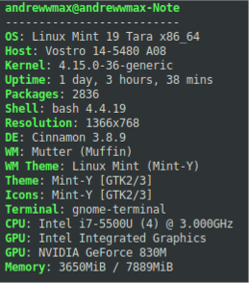
\includegraphics[scale=0.5]{Config.png}
% \caption{Neofetch}
% \label{fig_sim}
% \end{figure}

% \begin{listing}[ht]
% \begin{minted}[frame=lines, bgcolor=DarkGray, fontsize=\footnotesize, framesep=2mm, baselinestretch=1.2, breaklines,  breakanywhere]{c++}
% vector<string> sVazadas, sVerificar, sEncontradas;
% \end{minted}
% \caption{.................}
% \label{listing:1}
% \end{listing}

% \usemintedstyle{vim}
% \begin{listing}[ht]
% \begin{minted}[frame=lines, bgcolor=LightGray, fontsize=\footnotesize, framesep=2mm, baselinestretch=1.2, breaklines,  breakanywhere]{shell}

% env time -f "%C\n\tTempo de Execução:
%             %E\n\tMemória usada: %M\n"
%             -o memory.txt -a 
%             ./EP1......... 0 
%             txt/SenhasVazadas.txt txt/1000.txt

% ./EP1Seq 0 txt/SenhasVazadas.txt txt/1000.txt
%     Tempo de Execução: 0:36.17
%     Memória usada: 1051808

% ./EP1Paralel 4 txt/SenhasVazadas.txt txt/1000.txt
%     Tempo de Execução: 0:19.84
%     Memória usada: 1051772

% ./EP1BSTSeq 0 txt/SenhasVazadas.txt txt/1000.txt
%     Tempo de Execução: 0:11.28
%     Memória usada: 1051940

% ./EP1BSTParalel 4 txt/SenhasVazadas.txt txt/1000.txt
%     Tempo de Execução: 0:10.88
%     Memória usada: 1052048

% ./EP1Hash 0 txt/SenhasVazadas.txt txt/1000.txt
%     Tempo de Execução: 0:09.86
%     Memória usada: 1373080
        
% \end{minted}
% \caption{Resultados do teste de consumo de memória}
% \label{listing:6}
% \end{listing}

% \appendices
% \section{}

%%%%%%%%%%%%%%%%%%%%%%%%%%%%%%%%%%%%%%%%%%%%%%%%
% \begin{IEEEbiography}{André Thiago Borghi Couto}
% atualmente cursa graduação em Engenharia da Computação (2016/1) na Universidade Federal do Espírito Santo. Possui conhecimento em desenvolvimento de software, banco de dados, projetos em Arduino, design gráfico e tem interesse nos temas de automação em Arduino, inteligência artificial, redes de computadores e processamento de imagens.
% \end{IEEEbiography}

\newpage
\begin{IEEEbiographynophoto}{André Thiago Borghi Couto}
atualmente cursa graduação em Engenharia da Computação (2016/1) na Universidade Federal do Espírito Santo. Possui conhecimento em desenvolvimento de software, banco de dados, projetos em Arduino, design gráfico e tem interesse nos temas de automação em Arduino, inteligência artificial, redes de computadores e processamento de imagens.
\end{IEEEbiographynophoto}

\end{document}